\begin{figure}[H]
\centering
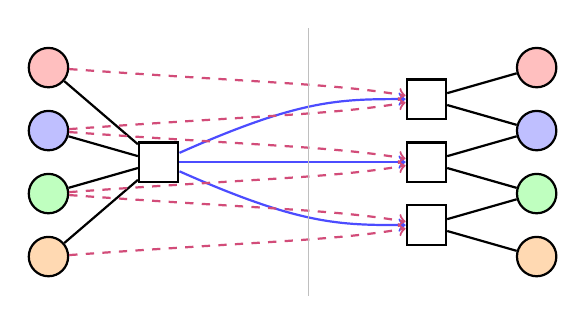
\begin{tikzpicture}[
    font=\small,
    % variable colors (consistent left/right)
    v1/.style={circle, draw, thick, fill=red!25,    minimum size=5mm, inner sep=0pt},
    v2/.style={circle, draw, thick, fill=blue!25,   minimum size=5mm, inner sep=0pt},
    v3/.style={circle, draw, thick, fill=green!25,  minimum size=5mm, inner sep=0pt},
    v4/.style={circle, draw, thick, fill=orange!30, minimum size=5mm, inner sep=0pt},
    fac/.style={rectangle, draw, thick, minimum size=5mm, inner sep=0pt},
    edge/.style={draw, thick},
    pred/.style={->, thick, draw=blue!70},
    map/.style={->, thick, dashed, draw=purple!70},
]

% -------------------------
% Left factor graph (high arity)
% -------------------------
\node[v1] (v1L) at (0,  1.2) {};
\node[v2] (v2L) at (0,  0.4) {};
\node[v3] (v3L) at (0, -0.4) {};
\node[v4] (v4L) at (0, -1.2) {};

\node[fac] (fHL) at (1.4, 0) {};

\foreach \v in {v1L,v2L,v3L,v4L}{
  \draw[edge] (\v) -- (fHL);
}

% -------------------------
% Right factor graph (low arity)
% -------------------------
\node[v1] (v1R) at (6.2,  1.2) {};
\node[v2] (v2R) at (6.2,  0.4) {};
\node[v3] (v3R) at (6.2, -0.4) {};
\node[v4] (v4R) at (6.2, -1.2) {};

\node[fac] (f12R) at (4.8,  0.8) {};
\node[fac] (f23R) at (4.8,  0.0) {};
\node[fac] (f34R) at (4.8, -0.8) {};

\draw[edge] (f12R) -- (v1R);
\draw[edge] (f12R) -- (v2R);

\draw[edge] (f23R) -- (v2R);
\draw[edge] (f23R) -- (v3R);

\draw[edge] (f34R) -- (v3R);
\draw[edge] (f34R) -- (v4R);

% -------------------------
% Precedence graph edges (colored, oriented)
% -------------------------
\draw[pred] (fHL) .. controls (3.2,  0.8) and (3.7,  0.8) .. (f12R);
\draw[pred] (fHL) .. controls (3.2,  0.0) and (3.7,  0.0) .. (f23R);
\draw[pred] (fHL) .. controls (3.2, -0.8) and (3.7, -0.8) .. (f34R);

% -------------------------
% Variable-to-factor mapping edges (dashed, oriented)
% -------------------------
\draw[map] (v1L) .. controls (2.8,  1.0) and (3.6,  1.0) .. (f12R);
\draw[map] (v2L) .. controls (2.8,  0.6) and (3.6,  0.6) .. (f12R);

\draw[map] (v2L) .. controls (2.8,  0.2) and (3.6,  0.2) .. (f23R);
\draw[map] (v3L) .. controls (2.8, -0.2) and (3.6, -0.2) .. (f23R);

\draw[map] (v3L) .. controls (2.8, -0.6) and (3.6, -0.6) .. (f34R);
\draw[map] (v4L) .. controls (2.8, -1.0) and (3.6, -1.0) .. (f34R);

% optional separator
\draw[draw=black!25] (3.3,1.7) -- (3.3,-1.7);

\end{tikzpicture}
\caption{Illustration of factor arity reduction.
Left: a single high-arity factor connected to four variables.
Right: a factor graph with only low-arity (pairwise) factors over the same variables.
Variable nodes share the same color across both graphs.
Colored arrows indicate \emph{precedence graph edges}, while dashed arrows indicate variable-to-factor mappings for pairwise factors sharing the same variables.}
\label{fig:chapter_5_factor_graph_precedence}
\end{figure}
